\begin{frame}{Main Problems: Robustness}
\begin{itemize}
    \item Training is sensitive to randomness in the environment, initialization of the policy and the algorithm implementation
\end{itemize}
\begin{figure}
    \centering
    
\includegraphics[width=0.7\textwidth,height=0.65\textheight,keepaspectratio]{images/soft-actor-critic/figures/walker-pair.jpg}
\end{figure}
\begin{flushright}
    \tiny\url{https://gym.openai.com/envs/Walker2d-v2/}
\end{flushright}
\end{frame}
\begin{frame}{Main Problems: Robustness}
\begin{itemize}
    \item Knowing only one way to act makes agents vulnerable to environmental changes that are common in the real-world
\end{itemize}
\begin{figure}
    \centering
    
\includegraphics[width=0.42\textwidth,height=0.6\textheight,keepaspectratio]{images/soft-actor-critic/figures/maze-left.jpg}\hspace{1em}
    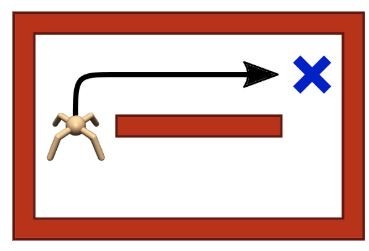
\includegraphics[width=0.42\textwidth,height=0.6\textheight,keepaspectratio]{images/soft-actor-critic/figures/maze-right.jpg}
\end{figure}
\begin{flushright}
    \tiny\url{https://bair.berkeley.edu/blog/2017/10/06/soft-q-learning/}
\end{flushright}
\end{frame}
